% Options for packages loaded elsewhere
\PassOptionsToPackage{unicode}{hyperref}
\PassOptionsToPackage{hyphens}{url}
%
\documentclass[
]{article}
\usepackage{amsmath,amssymb}
\usepackage{iftex}
\ifPDFTeX
  \usepackage[T1]{fontenc}
  \usepackage[utf8]{inputenc}
  \usepackage{textcomp} % provide euro and other symbols
\else % if luatex or xetex
  \usepackage{unicode-math} % this also loads fontspec
  \defaultfontfeatures{Scale=MatchLowercase}
  \defaultfontfeatures[\rmfamily]{Ligatures=TeX,Scale=1}
\fi
\usepackage{lmodern}
\ifPDFTeX\else
  % xetex/luatex font selection
\fi
% Use upquote if available, for straight quotes in verbatim environments
\IfFileExists{upquote.sty}{\usepackage{upquote}}{}
\IfFileExists{microtype.sty}{% use microtype if available
  \usepackage[]{microtype}
  \UseMicrotypeSet[protrusion]{basicmath} % disable protrusion for tt fonts
}{}
\makeatletter
\@ifundefined{KOMAClassName}{% if non-KOMA class
  \IfFileExists{parskip.sty}{%
    \usepackage{parskip}
  }{% else
    \setlength{\parindent}{0pt}
    \setlength{\parskip}{6pt plus 2pt minus 1pt}}
}{% if KOMA class
  \KOMAoptions{parskip=half}}
\makeatother
\usepackage{xcolor}
\usepackage[margin=1in]{geometry}
\usepackage{graphicx}
\makeatletter
\def\maxwidth{\ifdim\Gin@nat@width>\linewidth\linewidth\else\Gin@nat@width\fi}
\def\maxheight{\ifdim\Gin@nat@height>\textheight\textheight\else\Gin@nat@height\fi}
\makeatother
% Scale images if necessary, so that they will not overflow the page
% margins by default, and it is still possible to overwrite the defaults
% using explicit options in \includegraphics[width, height, ...]{}
\setkeys{Gin}{width=\maxwidth,height=\maxheight,keepaspectratio}
% Set default figure placement to htbp
\makeatletter
\def\fps@figure{htbp}
\makeatother
\setlength{\emergencystretch}{3em} % prevent overfull lines
\providecommand{\tightlist}{%
  \setlength{\itemsep}{0pt}\setlength{\parskip}{0pt}}
\setcounter{secnumdepth}{-\maxdimen} % remove section numbering
% definitions for citeproc citations
\NewDocumentCommand\citeproctext{}{}
\NewDocumentCommand\citeproc{mm}{%
  \begingroup\def\citeproctext{#2}\cite{#1}\endgroup}
\makeatletter
 % allow citations to break across lines
 \let\@cite@ofmt\@firstofone
 % avoid brackets around text for \cite:
 \def\@biblabel#1{}
 \def\@cite#1#2{{#1\if@tempswa , #2\fi}}
\makeatother
\newlength{\cslhangindent}
\setlength{\cslhangindent}{1.5em}
\newlength{\csllabelwidth}
\setlength{\csllabelwidth}{3em}
\newenvironment{CSLReferences}[2] % #1 hanging-indent, #2 entry-spacing
 {\begin{list}{}{%
  \setlength{\itemindent}{0pt}
  \setlength{\leftmargin}{0pt}
  \setlength{\parsep}{0pt}
  % turn on hanging indent if param 1 is 1
  \ifodd #1
   \setlength{\leftmargin}{\cslhangindent}
   \setlength{\itemindent}{-1\cslhangindent}
  \fi
  % set entry spacing
  \setlength{\itemsep}{#2\baselineskip}}}
 {\end{list}}
\usepackage{calc}
\newcommand{\CSLBlock}[1]{\hfill\break\parbox[t]{\linewidth}{\strut\ignorespaces#1\strut}}
\newcommand{\CSLLeftMargin}[1]{\parbox[t]{\csllabelwidth}{\strut#1\strut}}
\newcommand{\CSLRightInline}[1]{\parbox[t]{\linewidth - \csllabelwidth}{\strut#1\strut}}
\newcommand{\CSLIndent}[1]{\hspace{\cslhangindent}#1}
\usepackage{endfloat}
\usepackage{setspace}\doublespacing
\usepackage{lineno}
\linenumbers
\usepackage{rotating}
\ifLuaTeX
  \usepackage{selnolig}  % disable illegal ligatures
\fi
\usepackage{bookmark}
\IfFileExists{xurl.sty}{\usepackage{xurl}}{} % add URL line breaks if available
\urlstyle{same}
\hypersetup{
  pdftitle={BarnebyLives: an R package to create herbarium specimen labels and clean spreadsheets},
  pdfkeywords={herbarium, natural history museum, collections,
geospatial, R, LaTeX},
  hidelinks,
  pdfcreator={LaTeX via pandoc}}

\title{BarnebyLives: an R package to create herbarium specimen labels
and clean spreadsheets}
\author{Reed Clark Benkendorf\(^1\)\(^,\)\(^2\)\footnote{Author for
  Correspondence:
  \href{mailto:rbenkendorf@chicagobotanic.org}{\nolinkurl{rbenkendorf@chicagobotanic.org}}},
Jeremie B. Fant\(^1\)\(^,\)\(^2\)\\
\strut ~\(^1\)Chicago Botanic Garden, 1000 Lake Cook Road, Glencoe,
Illinois 60022, USA\\
\strut ~\(^2\)Plant Biology and Conservation, Northwestern University,
Evanston, Illinois 60208, USA}
\date{}

\begin{document}
\maketitle
\begin{abstract}
\noindent \textbf{Premise:} Accessioning herbarium specimens is
labor-intensive, yet remains vital for research in ecology, evolution,
and conservation. As institutional support for herbaria declines,
efficient tools are needed to streamline this process. BarnebyLives was
developed to assist collectors by supplementing collection notes,
verifying taxonomic data, conducting quality checks, generating labels,
and submitting digital records. \textbf{Methods and Results:} It
integrates geospatial data from U.S. government sources to provide
jurisdictional and site information, and checks taxonomic names using
in-house spell checkers, IPNI author standards, and Kew's Plants of the
World Online. Optional features include generating Google Maps driving
directions. The tool outputs data in tabular and spatial formats for
review before producing LaTeX-based labels and shipping manifests.\\
\textbf{Conclusions:} BarnebyLives improves data accuracy, ensures
up-to-date taxonomy, and significantly reduces the time and effort
required to accession herbarium specimens.
\end{abstract}

Nearly 400 million specimens are housed worldwide in herbaria
(\citeproc{ref-thiers2021herbaria}{Thiers, 2021}). However, The rate of
accessioning new collections to herbaria diminished in the
20\textsuperscript{th} century as priorities in biology shifted away
from describing and documenting earths biodiversity and towards
understanding cellular and molecular processes underpinning life
(\citeproc{ref-prather2004decline}{Prather et al., 2004};
\citeproc{ref-pyke2010biological}{Pyke and Ehrlich, 2010};
\citeproc{ref-daru2018widespread}{Daru et al., 2018}). This shift, among
other factors, led to a decline in the funding allocated to
collection-based research, the number of staff maintaining and accessing
new collections, and educating students in these practices
(\citeproc{ref-funk2014erosion}{Funk, 2014}). Historically, specimens
have been used to describe the taxonomic diversity of plants and
document global floristic diversity
(\citeproc{ref-greve2016realising}{Greve et al., 2016};
\citeproc{ref-james2018herbarium}{James et al., 2018};
\citeproc{ref-brewer2019factors}{Brewer et al., 2019};
\citeproc{ref-ronsted2020integrative}{Rønsted et al., 2020}). However,
renewed interest in herbarium collections utilizing `big data
approaches,' such as museuomics, has brought herbaria back to the
forefront of the natural sciences and grearly expanded their roles in
science (\citeproc{ref-ronsted2020integrative}{Rønsted et al., 2020};
\citeproc{ref-marsico2020small}{Marsico et al., 2020}).

Innovations in specimen digitization, data sharing, computing, DNA
sequencing, and statistics have perhaps brought about greater use of
herbarium specimens than ever before
(\citeproc{ref-greve2016realising}{Greve et al., 2016};
\citeproc{ref-james2018herbarium}{James et al., 2018};
\citeproc{ref-brewer2019factors}{Brewer et al., 2019};
\citeproc{ref-ronsted2020integrative}{Rønsted et al., 2020}). The
current use of specimens and their ancillary data extends well beyond
their traditional roles in systematics and floristics, and studies
utilizing collections are regularly carried out to better understand the
ecological niches, phenological processes, and interactions of plants
(\citeproc{ref-ronsted2020integrative}{Rønsted et al., 2020};
\citeproc{ref-davis2023herbarium}{Davis, 2023}). We suspect that
collections are yet to realize their full potential, and as currently
novel approaches, such as electronic and remote sensing and
meta-barcoding, become more accessible the use of collections will
increase (\citeproc{ref-tosa2021rapid}{Tosa et al., 2021}). While
image-based or purely observational (rather than collection-based)
citizen science approaches (e.g., iNaturalist, BudBurst) have recently
dovetailed with herbarium specimens to meet many current research needs,
specimens contain rich data that are not accessible via images. Only
specimens have the ability to: provide samples of DNA, secondary
metabolites, or proteins, material for measuring (micro-)morphological
attributes (\citeproc{ref-borges2020schrodinger}{Borges et al., 2020}),
and seeds or pollen. These factors will ensure that the specimens remain
the premier botanical data source into perpetuity.

However, despite renewed recognition of the utility of collections,
efforts to grow them appear slow
(\citeproc{ref-prather2004decline}{Prather et al., 2004}). We conjecture
that this is partly because collecting and depositing specimens is a
fundamentally slower process, especially for novice collectors, relative
to taking photographs via commercially developed apps on smartphones
(\citeproc{ref-daru2018widespread}{Daru et al., 2018};
\citeproc{ref-mishler2020spatial}{Mishler et al., 2020};
\citeproc{ref-manzano2021fair}{Manzano and Julier, 2021}). While many
young botanists are capable of using dichotomous keys and other
resources to reliably identify and collect satisfactory material, we
observe that they face difficulties navigating several aspects of data
acquisition, processing, and preparation of labels for submission to
herbaria. Some of the apparent problems include the lack of dedicated
time at the end of a field season to process specimens, a general lack
of education on cartography and orienteering, natural history (e.g.,
geology, geomorphology), nomenclature, and familiarity with various
computer programs (for example, Microsoft Office suite), and increasing
foundational knowledge of plant systematics and phylogenetics
(\citeproc{ref-woodland2007botanists}{Woodland, 2007};
\citeproc{ref-barrows2016crossroads}{Barrows et al., 2016};
\citeproc{ref-nanglu2023nature}{Nanglu et al., 2023}).

The generation of an herbarium specimen involves many steps that are
easy to take for granted (\citeproc{ref-forman1989herbarium}{Forman and
Bridson, 1989}). For example, while acquiring appropriate political
information for a collection site appears simple, young collectors
rarely have adequate cartographic resources (printed topographic maps or
GIS software) at their disposal. In topographically complex areas, where
administrative borders are often associated with hydrological basins and
the ridges defining them, collectors are liable to misinterpret their
true geographic position and report administrative details in error.
Even finding appropriate site names can rarely be resolved without a
printed map, as many navigation-related software now consider most
features that would serve as site names extraneous. Similarly, the rate
at which taxonomic innovations occur, the volume of the literature, and
the reluctance of some regional curators to embrace a phylogenetic
approach to plant classification have made it difficult to find more
recently applied scientific names, even when these names are unanimously
accepted by taxonomic specialists in the group and other regional
curators (\citeproc{ref-hitchcock2018flora}{Hitchcock and Cronquist,
2018}). Furthermore, formatting a label correctly (e.g., author
abbreviations, italicization, etc.) is a time-consuming process with
many opportunities to introduce errors in formatting which reduce the
apparent credibility of a collector. Anecdotally, many mail merge
templates offered by herbaria still require collectors to modify many
variables by hand, for example, applying italicization. Even if a
collector successfully navigates all these hurdles, the time allocated
to each step is quite large, and may discourage them from further
collecting.

As a result of these concerns, we have developed an R package,
BarnebyLives, that aims to increase both the quality of data rendered to
labels and recorded in databases and to speed up the generation of
labels. BarnebyLives rapidly provides political and administrative
boundary information for a collection site using data from the U.S.
Census Bureau (\citeproc{ref-walker2022tigris}{Walker, 2024}), the
Public Land Survey System (PLSS), and ownership details of public lands
via the Protected-Areas Database (PAD-US)
(\citeproc{ref-usgs2024padus}{Gap Analysis Project (GAP), 2024}). Site
names are suggested by finding the closest unambiguously named place
feature in the Geographic Name Information System (GNIS) and the precise
calculation of distance and azimuth from this feature to the collection
site (\citeproc{ref-gnis2024}{Survey, 2023}). Using the Global Mountain
Biodiversity Assessment (GMBA) Mountain Inventory V. 2, a standardized
named mountain data set with global coverage allows for a relevant
descriptor of the general region with less ambiguity
(\citeproc{ref-snethlage2022hierarchical}{Snethlage et al., 2022}).
Spell checks on all scientific names (including associated species) are
performed using a copy of the World Checklist of Vascular Plants, and
the resolved species may be searched via Kew's Plant of the World Online
for relevant synonyms (\citeproc{ref-govaerts2021world}{Govaerts et al.,
2021}; \citeproc{ref-powo2024}{POWO, 2024}). Author abbreviations are
verified using the International Plant Names Index (IPNI) Standard
Author Abbreviation Checklist and also returned by Kew's Plants of the
World Online to ensure proper abbreviations of authorities
(\citeproc{ref-ipni2024}{The Royal Botanic Gardens and Herbarium, 2024};
\citeproc{ref-powo2024}{POWO, 2024}). Checks to search for and flag
common issues associated with spreadsheet software or data
transcription, such as the auto-filling of coordinate and date columns.
After a final review of the data, flagged or generated by the package,
it allows for the option to export spreadsheets that are suitable for
mass uploading of data to multiple common herbarium databases as well as
the generation of herbarium labels.

Currently, to our knowledge label generation functionality is provided
explicitly by two programs, PLabel and Symbiota, and by the Microsoft
Word tool Mail Merge (\citeproc{ref-gries2014symbiota}{Gries et al.,
2014}; \citeproc{ref-perkins2020Plabel}{Perkins, 2020}). The office
suite costs money, and in our experience, is finicky; further, its
functionality ends with label creation. PLabel is a standalone program
that has greatly enhanced functionality relative to a mail merge,
allowing users to specify the layout and formatting of label components
using an intuitive and local graphical user interface (GUI)
functionality. However, beyond verifying the nations of collection it
does not include data cleaning functionalities.\\
While some sources indicate that it can only be used on Microsoft, we
expect it to be usable on Linux and Mac using Windows `emulators' like
Wine. The increasingly popular Symbiota biodiversity data management
software not only provides label generation capabilities but also
provides data cleaning functionality in an attractive GUI web portal
allowing for live management of collections and bypassing the need for a
local installation, allowing it to be accessed on all operating systems.
Symbiota offers functionality similar to the first four of our five
stages of our `Taxonomic' module and to our knowledge a check of the
`Political Boundaries' (see Figure 1). However, not all herbaria use
Symbiota and many have original database systems that they maintain (for
example, Harvard University Herbarium,
\url{https://kiki.huh.harvard.edu/databases/specimen_index.html};
Missouri Botanical Garden \url{https://tropicos.org/specimen/Search};
and The Consortium of Pacific Northwest Herbaria
\url{https://www.pnwherbaria.org/}). However, and most importantly many
collectors prefer to generate their own labels, especially as they are
likely to send different sets of collections to different institutions.
Accordingly, the functionality of Symbiota should exist in an ecosystem
with alternative systems. In scenarios where users want to keep
rendering labels in either of the three existing alternatives, they can
easily export data in the appropriate formats after utilizing BLs data
cleaning utilities.

BarnebyLives was named for plant taxonomist Rupert Charles Barneby
(1911-2000), who published over 6,500 pages of text, described over 750
taxa, and is notable for balancing his studies at the William and Lynda
Steere Herbarium at the New York Botanical Garden with annual collection
trips in Western North America from 1937-1970 and sporadically until he
passed in 2000 (\citeproc{ref-welsh2001rupert}{Welsh, 2001}). Select
accolades of Rupert include the 1989 Asa Gray Award from the American
Society of Plant Taxonomists (ASPT), the 1991 Engler Silver Medal from
the International Association of Plant Taxonomists (IAPT), as well as
being one of eight recipients of the International Botanical Congress's
(IBC) Millennium Botany Award (1999)
(\citeproc{ref-welsh2001rupert}{Welsh, 2001}). Most germanely, Rupert
was remembered as being generous with his time to assist younger
botanists with the more arcane aspects of field botany and taxonomy
(\citeproc{ref-holmgren2017}{Holmgren and Holmgren, 1988}).

\section{METHODS AND RESULTS}\label{methods-and-results}

\begin{figure}
\centering
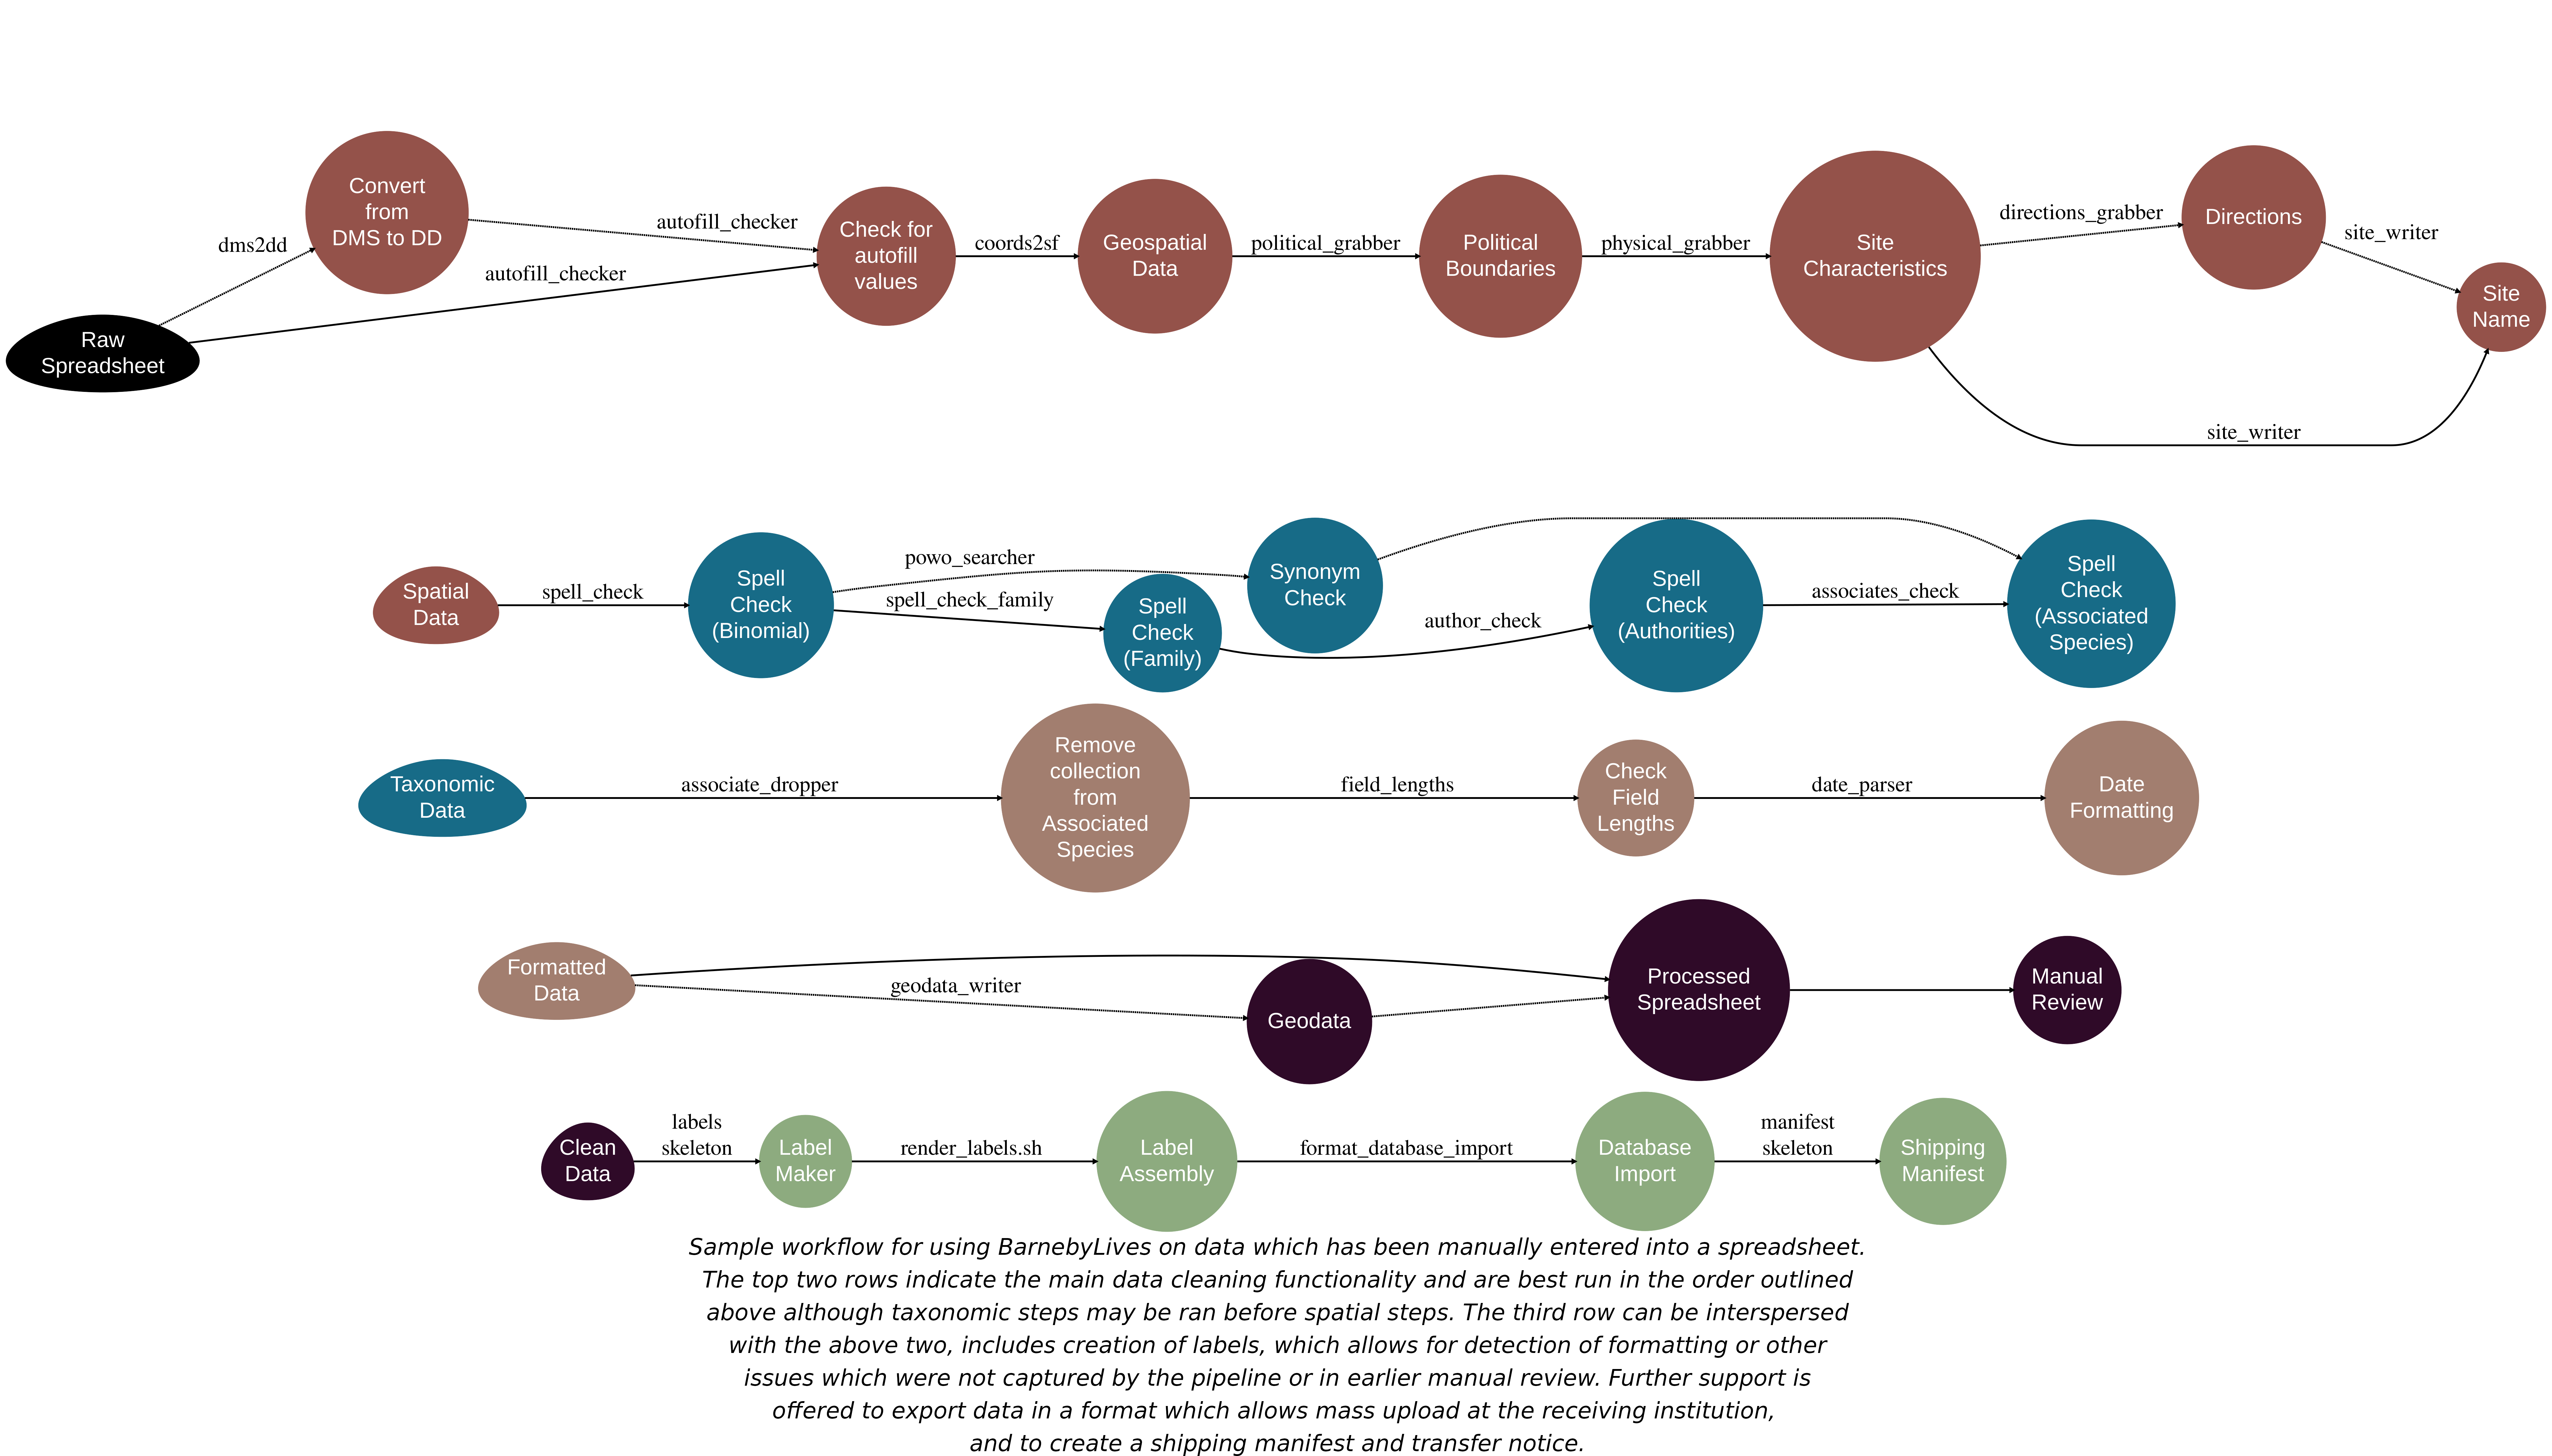
\includegraphics[width=1\textwidth,height=\textheight]{../graphics/plots/workflow.png}
\caption{Recommended workflow}
\end{figure}

BarnebyLives was iteratively developed based on data submitted by
approximately 20 seasonal field botany teams over two years.
Essentially, continual updates were made as the developers became aware
of the idiosyncrasies of collection notes and data entry. Several
commands in BarnebyLives require output from previous functions, and a
workflow that satisfies these requirements is presented in Figure 1.

\subsection{Usage}\label{usage}

All steps of BarnebyLives, except for label generation are run within
the freely available RStudio. Data may be read from any common
spreadsheet management system or database connection such as Excel, or
free alternatives such as LibreOffice, OpenOffice, or via the cloud on
Google Sheets. The latter two options are documented here and in package
vignettes, detailed descriptions of the required and suggested input
columns are located on a Github Pages
(\url{https://sagesteppe.github.io/BarnebyLives/}) and around 100
real-world examples are on a Google Sheets accessible from the page.
BarnebyLives is atypical for R packages in that it requires a
considerable amount of data to operate (Table 1). Virtually all on-disk
memory associated with the package are used to store spatial data. The
amount of spatial data varies according to the domain that the user
decides to support (Figure 3). Functions that require on-disk data
require a path to data as an argument. Manually supplying the path
argument allows users to determine an appropriate storage location
suitable for their needs.

We anticipate that for a typical user, BarnebyLives will require less
than a couple gigabytes of memory (ours covering all of the conterminous
Western U.S. at 3-arc second (\textasciitilde90m) resolution is
\textasciitilde16 GiB), while the processing requires relatively little
RAM; hence, we believe installations can work on hardware as limited as
Chromebooks, while having the data stored entirely on thumb-drives.
Given that the attributes which the package collects data on are
tailored to the Western U.S. region, we do not expect local installs to
exceed the size of ours. The final steps of BarnebyLives, generating the
labels, requires working installations of R Markdown, a LaTeX
installation
(e.g.~\href{https://www.tug.org/applications/pdftex/}{pdfTeX},
\href{https://www.luatex.org/}{LuaTeX},
\href{https://www.overleaf.com/learn/latex/XeLaTeX}{XeLaTeX}), and the
open source command line tools
\href{https://github.com/rrthomas/pdfjam}{pdfjam} and
\href{https://linux.die.net/man/1/pdftk}{pdftk}. While these steps are
run through a shell scripting language such as bash, we have wrapped
them in R functions that bypass the need to enter the commands directly
into a shell terminal outside of RStudio. Unfortunately, we have not
found Windows alternatives to pdfam and pdftek, so we are unable to
offer the final label-generating functionality on that operating system,
but suspect Ubuntu subsystem for Windows may allow for integration of
these tools.

\subsection{Functionality}\label{functionality}

BarnebyLives can be thought of as consisting of five main modules
(Figure 1): spatial, taxonomic, formatting, manual review, and data
exporting.

The spatial module has five required functions and two optional
functions.\\
\emph{autofill\_checker} searches for patterns in the input latitude and
longitude data associated with autofilling from various spreadsheet
programs and will emit a warning if they are encountered.\\
\emph{coords2sf} creates a spatially explicit simple feature (sf)
geometry dataset for the input data. \emph{political\_grabber}
determines many levels of administrative ownership, including land
management and public land survey system sections.\\
\emph{physical\_grabber} provides various geographic data, such as
elevation, landform position, and aspect using 90m resolution spatial
data.\\
\emph{site\_writer} write distance and azimuth to collection site from
the nearest official named place from the GNIS database.
\emph{directions\_grabber} is an optional function that writes driving
directions from a reasonably sized town to the closest drivable area to
the site using the Google Maps API, which will require a valid Google
account that is free per month for most personal and smaller academic
usages.\\
\emph{dms2dd} is an optional function used to convert from coordinates
denoted in the degrees minutes and second format (for example,
42°08'39.9"N 87°47'08.3"W) to decimal degree format (for example
42.14439, -87.78569).

Please note that the function \emph{physical\_grabber} is the one
portion of the package where a decoupling may exist between the
collection site, and the resolution of the spatial data. While we expect
the mismatch to be negligible for all effective purposes relating to:
elevation, major geology type, and in general aspect, estimates of slope
at this resolution may be biased - generally to lower angles. For these
reasons collectors must always make notes on the truly local environment
which taxa are found in, and consider that the notes from BL reflect the
greater landscape which a microfeature may be present in. While this
mis-match will seldom effect landscape ecologists, it may have
implications for other data users.

The taxonomic module has four required functions and one optional
function.\\
\emph{spell\_check} will perform a spell check on the entered scientific
name based on a local copy of Kew Plants of the World database filtered
to the local continents or a user-specified backbone.\\
\emph{spell\_check\_family} performs a spell check on the family entered
for each scientific name.\\
\emph{author\_check} ensures that the authors are entered in a valid
format, for example, the correct standard abbreviations are used.\\
\emph{associates\_check} performs a spell check on all associated
species using the local taxonomic database. \emph{powo\_searcher} can be
used in tandem with the functions \emph{spell\_check\_family} and
\emph{author\_check}, but we use it in lieu of them to search the
current Plants of the World Online to determine relevant synonyms and
alternative higher taxonomy for the focal species. No API key or
registration is required to use \emph{powo\_searcher}.

The formatting module has three functions. Two are optional; however,
they are run locally and so quickly that there is no reason to skip
them. \emph{date\_parser} parses an input date into various formats for
notating collection and determination dates on labels.
\emph{associate\_dropper} silently removes the collected species from
the list of associated species; however, it searches for the species to
be removed using the scientific name entered initially by the user
rather than returned via spell checks. \emph{field\_lengths} will emit
messages for any fields that we suspect will create an `overflow' on the
physical label and should be truncated for clarity.

The manual review process technically only has one function that is
optional and may be executed during the spatial process (after
\emph{coords2sf}), but the importance of manual review is important
enough to warrant explicit mention.\\
\emph{geodata\_writer} will write out a spatial copy of the data set to
any geospatial format supported by the sf package, but defaults to
writing out `kmls' which are readily used with
\href{https://earth.google.com/web/}{Google Earth}, and can also be
opened in several other free geographic information system (GIS)
softwares such as \href{https://www.qgis.org/}{QGIS}. Notably, many of
the flags that BarnebyLives generates will be placed into columns with
obviously flagged names and can be manually reviewed by the analyst, and
many of these issues can be resolved by simply addressing the relevant
issues in the original data input spreadsheet.

The data exporting module contains three functions that interact with
LaTeX templates and require slightly more advanced R user interactivity,
such as setting up mapping functions using the tidyverses purrr
package.\\
\emph{labels\_skeleton} is an R `script' which will require a few
modification steps to tailor to each institution, these R scripts will
put data into a user specified template, and serve as the interface to
LaTeX.\\
\emph{label\_writer} write from a flatfile or spreadsheet to small 4x4
inch herbarium labels (users can modify these dimensions as they see
fit). \emph{format\_database\_import} will write out a spreadsheet of
cleaned data in a variety of formats, currently: Jepson, Symbiota, and
Consortium of Pacific Northwest herbaria are supported.

\subsubsection{Herbarium Collections}\label{herbarium-collections}

\begin{figure}
\centering
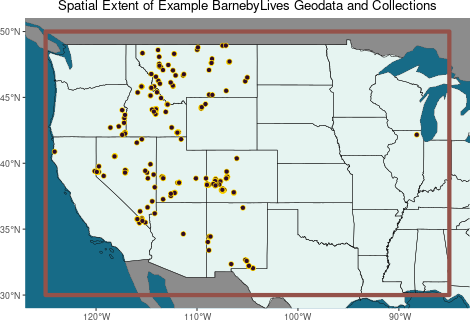
\includegraphics[width=0.5\textwidth,height=\textheight]{../graphics/plots/collections_map.png}
\caption{The spatial extent-or domain- (orange), and herbarium
collection sites (burgundy) tested in this manuscript.}
\end{figure}

The testing of the package within this manuscript was performed using a
subset of the authors collections from 2018-2022, while most development
was performed on their 2023 and 2024 collections. Only collections which
had identifications to the level of species or lower, and transcribed
collection dates and coordinates were used for most functionality. In
total 981 records were used for testing various functions, these records
were from 234 sites located across Western North America (Figure 2). In
total this data set had 729 species (with 558 distinct sets of authors),
with 83 infraspecies (22 authorships) in 74 families.

BarnebyLives took roughly four minutes (222.886sec) to run all local
steps, and roughly ten minutes (584.05sec) to search Plants of the World
Online for preferred synonyms, and a minute 63.945sec to search Google
Maps and write directions to sites.

Most of the local run time is attributable to the spatial (205.254sec),
and taxonomic operations (17.253sec), while formatting data for labels
took 0.379sec. The spell check of the scientific name accounted for
nearly all of the time (17.006sec) spent performing local taxonomic
operations. The generation of labels consumed around eight minutes
(509.931sec) for the rendering, and an additional 58.60sec to combine
the 182 sheets to a single Portable Document Format (PDF). The total
label generation run time for processing these 729 collections was 15
minutes. In total the 729 collections, which underwent all processing
steps, took 24 minutes to process.

\subsection{RESULTS}\label{results}

Even on data which had been manually cleaned and error-checked by a
human several times BarnebyLives was able to reduce transcription
errors, identify typos, make nomenclature suggestions, and reformat text
elements for downstream use. While none of the 74 families were
misspelled, BarnebyLives made 25 suggestions on naming, identified 6
instances where the user entered an unequivocally incorrect family (or
taxonomic entity), identified 5 records where families were autofilled,
and 1 instance where an outdated circumscription was applied. At the
level of family BarnebyLives flagged 6 records where the author follows
an alternative taxonomy, and flagged 7 records in error, it appears most
of these errors are due to issues in the backbone used by the earlier
spell check function.

In the 326 genera analysed BarnebyLives identified 75 discrepancies at
the level of genus between user submitted and processed data. In 42 of
these instances the user supplied an outdated name (21 unique genera)
flagged 4 records where the author follows an alternative taxonomy (2
genera total), and flagged 2 record in error.

Of 729 distinct species analysed BarnebyLives flagged 61 records, and
detected 33 instances of misspelled epithets (33 unique species). In 15
of these instances the user supplied an outdated name (15 unique
species). It also flagged 2 records where the author follows an
alternative taxonomy (2 unique species), and flagged 8 records in error.
The final record was an egregious error where the order of the specific
epithet and the genus name.

5 records were appropriately flagged for issues with auto fill increment
of the longitude value, and 3 records were also auto-flagged for
increases in latitude values.

\begin{figure}
\centering
\includegraphics[width=0.5\textwidth,height=\textheight]{../graphics/tables/Screenshot-DataSources.png}
\caption{Data Sources}
\end{figure}

\section{DISCUSSION}\label{discussion}

While numerous tools have been developed for cleaning existing herbarium
and museum records, few tools help to ensure that the data entered are
accurate (\citeproc{ref-patten2024geographic}{Patten et al., 2024}). We
argue that the original collectors are the most qualified individuals to
perform quality control checks and that BarnebyLives allows them to
assume that responsibility in a relatively fast and streamlined format.
By utilizing both R and LaTeX and having publicly available source code
on Github, this program allows users immediate familiarity with the
system for troubleshooting issues and implementing upgrades and
modifications in project branches.

LaTeX, a software system used for typesetting, allows users to focus on
the content rather than the style of the documents rendered from it.
However, using its default settings, it can produce aesthetically
pleasing results (Figure 4). Additionally LaTeX offers users a wide
variety of ways which they can modify labels which are under-explored in
the package. Very good documentation of LaTeX capabilities is offered in
multiple areas; for instance, via the
\href{https://www.overleaf.com/learn}{Overleaf} project. While the
templates in the package are quite simple, LaTeX also offers the ability
to use custom fonts, to alter font weights and colors, alter line
spacing, to include images (e.g.~dot maps) and customize labels beyond
what the default templates support.

Thematically, BarnebyLives is set up to cover Western North America.
However, the package supports the use of a `domain' being drawn over any
of the conterminous United States. Several of the attributes which it
collects and displays on labels, relate to topics which more senior
curators are interested in, i.e.~the administrative information on
Township Section and Range (or `TRS'), but are considered less value in
other geographic regions.\\
Further several of the abiotic variables which it acquires information
on: slope, aspect, and geology have long been considered prominent
drivers of plant distributions in semi-arid and montane systems and
warranted on a label in these types of systems, whereas curators in
other regions may find this information superfluous. Finally, it is
plausible people in other geographic areas are less interested in
displaying which land management agency has jurisdiction over a
collection; however in the west we believe this is useful information
which may help a collector interested in revisiting a site to determine
if they will require permits for access or to make new collections.

Accessioning often relies on the use of the Microsoft Office suite of
programs and may utilize other costly software such as ArcPro or Adobe
Acrobat. While BarnebyLives does not have its own graphic user
interface, the functionality of commonly used Interactive Development
Environments (IDE's), such as Rstudio and VisualStudio (VS) Code, now
offer functionality to readily view and filter datasets using familiar
spreadsheet-like formats, making them more accessible to many users.
While other software often cost money, these are also free, and we
recommend that users install an open-source PDF viewer such as Okular to
review their rendered documents.

\begin{figure}
\centering
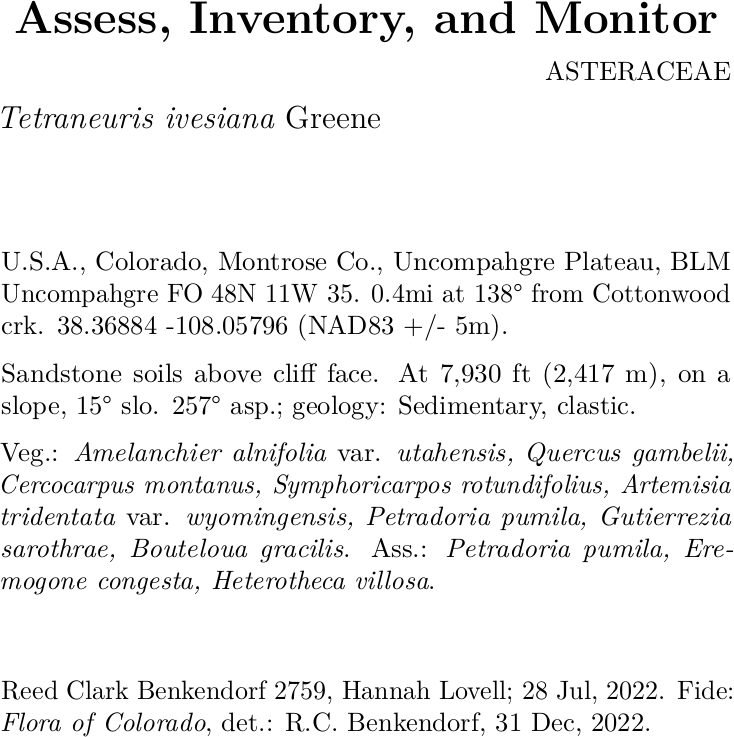
\includegraphics[width=0.5\textwidth,height=\textheight]{../graphics/plots/RCB2759.png}
\caption{A label generated from a default template}
\end{figure}

\section{CONCLUSIONS}\label{conclusions}

BarnebyLives is an R package that can be used to rapidly acquire
relevant geographic and taxonomic data. It can also perform specialized
spell checks and assorted curatorial tasks to produce both digital and
analog data. The package relies on no licensed software, such as the
Microsoft Office suite, and is suitable for install on all major
operating systems (Windows, Mac, Linux), however currently label
generation support is only offered on Linux and Mac, with a small amount
of use of the command line, which may be called from the Rstudio rather
than a `traditional' terminal.

\section{AUTHOR CONTRIBUTIONS}\label{author-contributions}

The project was conceptualized by R.C.B. The program was written by
R.C.B. Data collection and analysis were performed by R.C.B. R.C.B. \&
J.B.F wrote the manuscript, and both authors approved the final version
of the manuscript.

\section{ACKNOWLEDGEMENTS}\label{acknowledgements}

The Bureau of Land Management is gratefully acknowledged as a provider
of funding to R.C.B. for most of his specimen collection activities. We
thank the two anonymous peer reviewers who have increased the quality of
this manuscript. Several prominent associated collectors of specimens
used in this study are thanked: Dani Yashinovitz, Hannah Lovell, Dakota
Becerra, Caitlin Miller, Hubert Szczygiel.

\section{DATA AVAILABILITY STATEMENT}\label{data-availability-statement}

The BarnebyLives R package is open source, the development version is
available on GitHub (\url{https://github.com/sagesteppe/BarnebyLives}).
The package includes three real use-case vignettes (tutorials) available
on a Github Pages site
(\url{https://sagesteppe.github.io/BarnebyLives/}). The first vignette
\emph{``Preparing to use BarnebyLives!''} shows how to set up an
instance for a certain geographic area (domain). The next two vignettes
\emph{``BarnebyLives! Running pipeline''} showcases the usage of the
package for processing data entered on a spreadsheet, and
\emph{``Printing herbarium labels and exporting a digital copy of
data''} how to export data in both digital and analog formats.
\emph{``Custom label templates''} shows how to customize labels in
LaTeX, and \emph{``Rendering a shipping manifest''} details how to
produce a shipping manifest for gifting or transferring material to an
herbarium. All data used in this manuscript are available at:
\url{https://github.com/sagesteppe/Barneby_Lives_dev/manuscript}.

\singlespacing

\section{ORCID}\label{orcid}

Reed Clark Benkendorf \url{https://orcid.org/0000-0003-3110-6687}\\
Jeremie Fant \url{https://orcid.org/0000-0001-9276-1111}

\small

\section{REFERENCES}\label{references}

\clearpage

\phantomsection\label{refs}
\begin{CSLReferences}{1}{1}
\bibitem[\citeproctext]{ref-barrows2016crossroads}
Barrows, C. W., M. L. Murphy-Mariscal, and R. R. Hernandez. 2016. At a
crossroads: The nature of natural history in the twenty-first century.
\emph{BioScience} 66: 592--599.

\bibitem[\citeproctext]{ref-borges2020schrodinger}
Borges, L. M., V. C. Reis, and R. Izbicki. 2020. Schrodinger's
phenotypes: Herbarium specimens show two-dimensional images are both
good and (not so) bad sources of morphological data. \emph{Methods in
Ecology and Evolution} 11: 1296--1308.

\bibitem[\citeproctext]{ref-brewer2019factors}
Brewer, G. E., J. J. Clarkson, O. Maurin, A. R. Zuntini, V. Barber, S.
Bellot, N. Biggs, et al. 2019. Factors affecting targeted sequencing of
353 nuclear genes from herbarium specimens spanning the diversity of
angiosperms. \emph{Frontiers in plant science} 10: 1102.

\bibitem[\citeproctext]{ref-daru2018widespread}
Daru, B. H., D. S. Park, R. B. Primack, C. G. Willis, D. S. Barrington,
T. J. Whitfeld, T. G. Seidler, et al. 2018. Widespread sampling biases
in herbaria revealed from large-scale digitization. \emph{New
Phytologist} 217: 939--955.

\bibitem[\citeproctext]{ref-davis2023herbarium}
Davis, C. C. 2023. The herbarium of the future. \emph{Trends in Ecology
\& Evolution} 38: 412--423.

\bibitem[\citeproctext]{ref-forman1989herbarium}
Forman, L., and D. Bridson. 1989. The herbarium handbook. Royal Botanic
Gardens Kew.

\bibitem[\citeproctext]{ref-funk2014erosion}
Funk, V. A. 2014. The erosion of collections-based science: Alarming
trend or coincidence. \emph{The Plant Press} 17: 1--13.

\bibitem[\citeproctext]{ref-usgs2024padus}
Gap Analysis Project (GAP), U. S. G. S. (USGS). 2024. Protected areas
database of the united states (PAD-US) 4.0.

\bibitem[\citeproctext]{ref-govaerts2021world}
Govaerts, R., E. Nic Lughadha, N. Black, R. Turner, and A. Paton. 2021.
The world checklist of vascular plants, a continuously updated resource
for exploring global plant diversity. \emph{Scientific data} 8: 215.

\bibitem[\citeproctext]{ref-greve2016realising}
Greve, M., A. M. Lykke, C. W. Fagg, R. E. Gereau, G. P. Lewis, R.
Marchant, A. R. Marshall, et al. 2016. Realising the potential of
herbarium records for conservation biology. \emph{South African Journal
of Botany} 105: 317--323.

\bibitem[\citeproctext]{ref-gries2014symbiota}
Gries, C., M. E. E. Gilbert, and N. M. Franz. 2014. Symbiota--a virtual
platform for creating voucher-based biodiversity information
communities. \emph{Biodiversity data journal}.

\bibitem[\citeproctext]{ref-hitchcock2018flora}
Hitchcock, C. L., and A. Cronquist. 2018. Flora of the pacific
northwest: An illustrated manual. University of Washington Press.

\bibitem[\citeproctext]{ref-holmgren2017}
Holmgren, N., and P. Holmgren. 1988. Intermountain flora v. 7. The New
York Botanical Garden Press, New York.

\bibitem[\citeproctext]{ref-james2018herbarium}
James, S. A., P. S. Soltis, L. Belbin, A. D. Chapman, G. Nelson, D. L.
Paul, and M. Collins. 2018. Herbarium data: Global biodiversity and
societal botanical needs for novel research. \emph{Applications in plant
sciences} 6: e1024.

\bibitem[\citeproctext]{ref-manzano2021fair}
Manzano, S., and A. C. Julier. 2021. How FAIR are plant sciences in the
twenty-first century? The pressing need for reproducibility in plant
ecology and evolution. \emph{Proceedings of the Royal Society B} 288:
20202597.

\bibitem[\citeproctext]{ref-marsico2020small}
Marsico, T. D., E. R. Krimmel, J. R. Carter, E. L. Gillespie, P. D.
Lowe, R. McCauley, A. B. Morris, et al. 2020. Small herbaria contribute
unique biogeographic records to county, locality, and temporal scales.
\emph{American journal of botany} 107: 1577--1587.

\bibitem[\citeproctext]{ref-mishler2020spatial}
Mishler, B. D., R. Guralnick, P. S. Soltis, S. A. Smith, D. E. Soltis,
N. Barve, J. M. Allen, and S. W. Laffan. 2020. Spatial phylogenetics of
the north american flora. \emph{Journal of Systematics and Evolution}
58: 393--405.

\bibitem[\citeproctext]{ref-nanglu2023nature}
Nanglu, K., D. de Carle, T. M. Cullen, E. B. Anderson, S. Arif, R. A.
Castañeda, L. M. Chang, et al. 2023. The nature of science: The
fundamental role of natural history in ecology, evolution, conservation,
and education. \emph{Ecology and Evolution} 13: e10621.

\bibitem[\citeproctext]{ref-patten2024geographic}
Patten, N. N., M. L. Gaynor, D. E. Soltis, and P. S. Soltis. 2024.
Geographic and taxonomic occurrence r-based scrubbing (gatoRs): An r
package and workflow for processing biodiversity data.
\emph{Applications in Plant Sciences} 12: e11575.

\bibitem[\citeproctext]{ref-perkins2020Plabel}
Perkins, K. 2020. Plabel.

\bibitem[\citeproctext]{ref-powo2024}
POWO. 2024. Geographic names information system (GNIS) - USGS national
map downloadable data collection: U.s. Geological survey.

\bibitem[\citeproctext]{ref-prather2004decline}
Prather, L. A., O. Alvarez-Fuentes, M. H. Mayfield, and C. J. Ferguson.
2004. The decline of plant collecting in the united states: A threat to
the infrastructure of biodiversity studies. \emph{Systematic Botany} 29:
15--28.

\bibitem[\citeproctext]{ref-pyke2010biological}
Pyke, G. H., and P. R. Ehrlich. 2010. Biological collections and
ecological/environmental research: A review, some observations and a
look to the future. \emph{Biological reviews} 85: 247--266.

\bibitem[\citeproctext]{ref-ronsted2020integrative}
Rønsted, N., O. M. Grace, and M. A. Carine. 2020. Integrative and
translational uses of herbarium collections across time, space, and
species. \emph{Frontiers in Plant Science} 11: 1319.

\bibitem[\citeproctext]{ref-snethlage2022hierarchical}
Snethlage, M. A., J. Geschke, A. Ranipeta, W. Jetz, N. G. Yoccoz, C.
Körner, E. M. Spehn, et al. 2022. A hierarchical inventory of the
world's mountains for global comparative mountain science.
\emph{Scientific data} 9: 149.

\bibitem[\citeproctext]{ref-gnis2024}
Survey, U. S. G. 2023. Geographic names information system (GNIS) - USGS
national map downloadable data collection: U.s. Geological survey.

\bibitem[\citeproctext]{ref-ipni2024}
The Royal Botanic Gardens, H. U. H. \&. L., Kew, and A. N. Herbarium.
2024. International plant names index.

\bibitem[\citeproctext]{ref-thiers2021herbaria}
Thiers, B. M. 2021. The world's herbaria 2021: A summary report based on
data from index herbarium.

\bibitem[\citeproctext]{ref-tosa2021rapid}
Tosa, M. I., E. H. Dziedzic, C. L. Appel, J. Urbina, A. Massey, J.
Ruprecht, C. E. Eriksson, et al. 2021. The rapid rise of next-generation
natural history. \emph{Frontiers in Ecology and Evolution} 9: 698131.

\bibitem[\citeproctext]{ref-walker2022tigris}
Walker, K. 2024.
\href{https://CRAN.R-project.org/package=tigris}{Tigris: Load census
TIGER/line shapefiles}.

\bibitem[\citeproctext]{ref-welsh2001rupert}
Welsh, S. L. 2001. Rupert c. Barneby (1911-2000). \emph{Taxon}.

\bibitem[\citeproctext]{ref-woodland2007botanists}
Woodland, D. W. 2007. Are botanists becoming the dinosaurs of biology in
the 21st century? \emph{South African Journal of Botany} 73: 343--346.

\end{CSLReferences}

\section{SUPPORTING INFORMATION}\label{supporting-information}

Additional supporting information can be found online in the Supporting
Information section at the end of this article.

\textbf{Appendix S1.} A table of all time trials for each function.

\end{document}
